\documentclass{article}

\usepackage{graphicx}
\pagestyle{plain}
\usepackage[utf8]{inputenc}
\usepackage[T1]{fontenc}
\usepackage[unicode]{hyperref}

\author{Patryk Jędrzejko 200406}
\title{Sprawozdanie z laboratorium - PAiMSI. \\Algorytmy sortowania.}

\begin{document}
\maketitle

\section{Wprowadzenie}
Celem ćwiczenia było napisanie programu, który będzie zawierał algorytmy sortowania, a następnie zbadanie złożoności obliczeniowej dla sortowania wczytanych danych z pliku. Program został napisany na podstawie wcześniejszej klasy Kolejka. Jest to klasa kolejki jako tablica.
Kolejno algorytmy sortowały ilość elementów n = 10, 100, 1000, 10000,100000.
\\\\Wybrane algorytmy sortowania:
\begin{itemize}
  \item \textbf{QuickSort} - czyli szybkiego sortowania,
  \item \textbf{MergeSort} - sortowanie przez scalanie,
  \item \textbf{HeapSort} - sortowanie kopcem.
\end{itemize}
\section{Opis poszczególnych algorytmów sortowania}
Pierwszy z nich algorytm QuickSort jest przykładem zastosowania techniki "dziel i zwyciężaj" i składa się z 3 faz: 1.najpierw wejściowy ciąg liczb jest dzielony na dwa podciągi, 2. następnie te dwa podciągi są sortowane rekurencyjnie, 3. posortowane podciągi scala się w jeden posortowany ciąg.
\\\\Algorytm MergeSort jest jednym z prostrzych przykładów zastosowania wyżej wymienionej techniki "dziel i zwyciężaj", to znaczy: 1. dzieli ciąg na dwa ciągi o długości n/2, 2. sortuje te dwa ciągi przy użyciu sortowania przez scalanie, 3. posortowane ciągi długości n/2 scala w posortowany ciąg długości n.
\\\\Trzeci algorytm sortowania HeapSort, czyli sortowanie przez kopcowanie opiera się na stworzeniu kopca, a następnie na rozbiorze utworzonego kopca, w wyniku czego otrzymujemy posortowany ciąg.
\section{Analiza złożoności algorytmów sortowania:}
\begin{itemize}
  \item Dla algorytmu MergeSort oraz HeapSort klasa złożoności wynosi O(n logn) dla elementów losowych, posortowanych jak i posortowanych malejąco.
  \item Ważnym elementem w sortowaniu szybkim jest wybór pivota, czyli elementu rozdzielającego. Aby uchronić algorytm QuickSort przed złożonością $ O(n^{2}) $ - jest to przypadek, gdy element podziału zostaje ustalony jako element skrajny tablicy - należy randomizować element podziału, aby nasz algorytm szukania był optymalny. Jednym ze sposobów aby uniknąć złożoności pesymistycznej jest dodanie do algorytmu szukanie mediany, która dzieli naszą tablicę. Jak również wybór z pomiędzy trzech elementów, które są jako środkowe i z nich wybrać element osiowy, czyli taki, który leży pomiędzy nimi. I w taki sposób możemy uzyskać prawdopodobieństwo zajścia najgorszego przypadku do wartości zaniedbywalnie małych.
  \item Klasa złożoności obliczeniowej dla algorytmu QuickSort dla elementów posortowanych malejąco oraz posortowanych wynosi $ O(n^{2}) $  czyli dla najgorszego przypadku (złożoność pesymistyczna), zaś dla najlepszego przypadku klasa złożoności przyjmuje wartość O(n logn) dla elementów losowych (złożoność optymistyczna oraz typowa). Przez co możemy określić iż sortowanie szybkie nie jest sortowaniem stabilnym.
\end{itemize}
\section{Wnioski:}
Analizując wyniki obliczeń w arkuszu kalkulacyjnym otrzymanych czasów sortowania użytych algorytmów możemy wyciągnąć wnioski takie, że:
\begin{itemize}
    \item Porównując czasy wykonania sortowania dla różnych ilości n elementów do posortowania widzimy, że dla małej liczby elementów tj. n = 10, to są różnice nieznaczne, zaś dla n = 100000 elementów możemy już stwierdzić różnicę czasową w wykonaniu sortowania dla elementów losowych.
  \item Następnie możemy odczytać z tabeli, że dla sortowania przez scalanie dla elementów losowych algorytm jest najwolniejszy. Dla elementów posortowanych malejąco algorytm wykonuje sortowanie najszybciej.
  \item Zaś dla sortowania szybkiego widzimy znaczące zmiany dla elementów posortowanych i malejących, co może wynikać z nieprawidłowego wykonania algorytmu sortowania bądź też niestabilności sortowania szybkiego. Znaczące zmiany widzimy już dla n = 1000. Dlatego QuickSort jest najszybszy dla elementów losowych.
  \item Dla sortowania przez kopcowanie mamy podobnie jak z SortMerge. Widzimy, że dla elementów posortowanych sortowanie wykonuje się najszybciej, zaś dla malejących najwolniej.
  \item Możemy zatem stwierdzić, iż algorytm szybkiego sortowania jest najszybszy, ale tylko dla elementów losowych. Zaś najwolniejszym z nich jest algorytm kopcowania. Co za tym idzie algorytm QuickSort jest efektywniejszy od pozostałych algorytmów sortowania.
\end{itemize}
\textbf{Tabela wyników oraz wykresy na stronie 4 oraz 5.}
\begin{figure}[H]
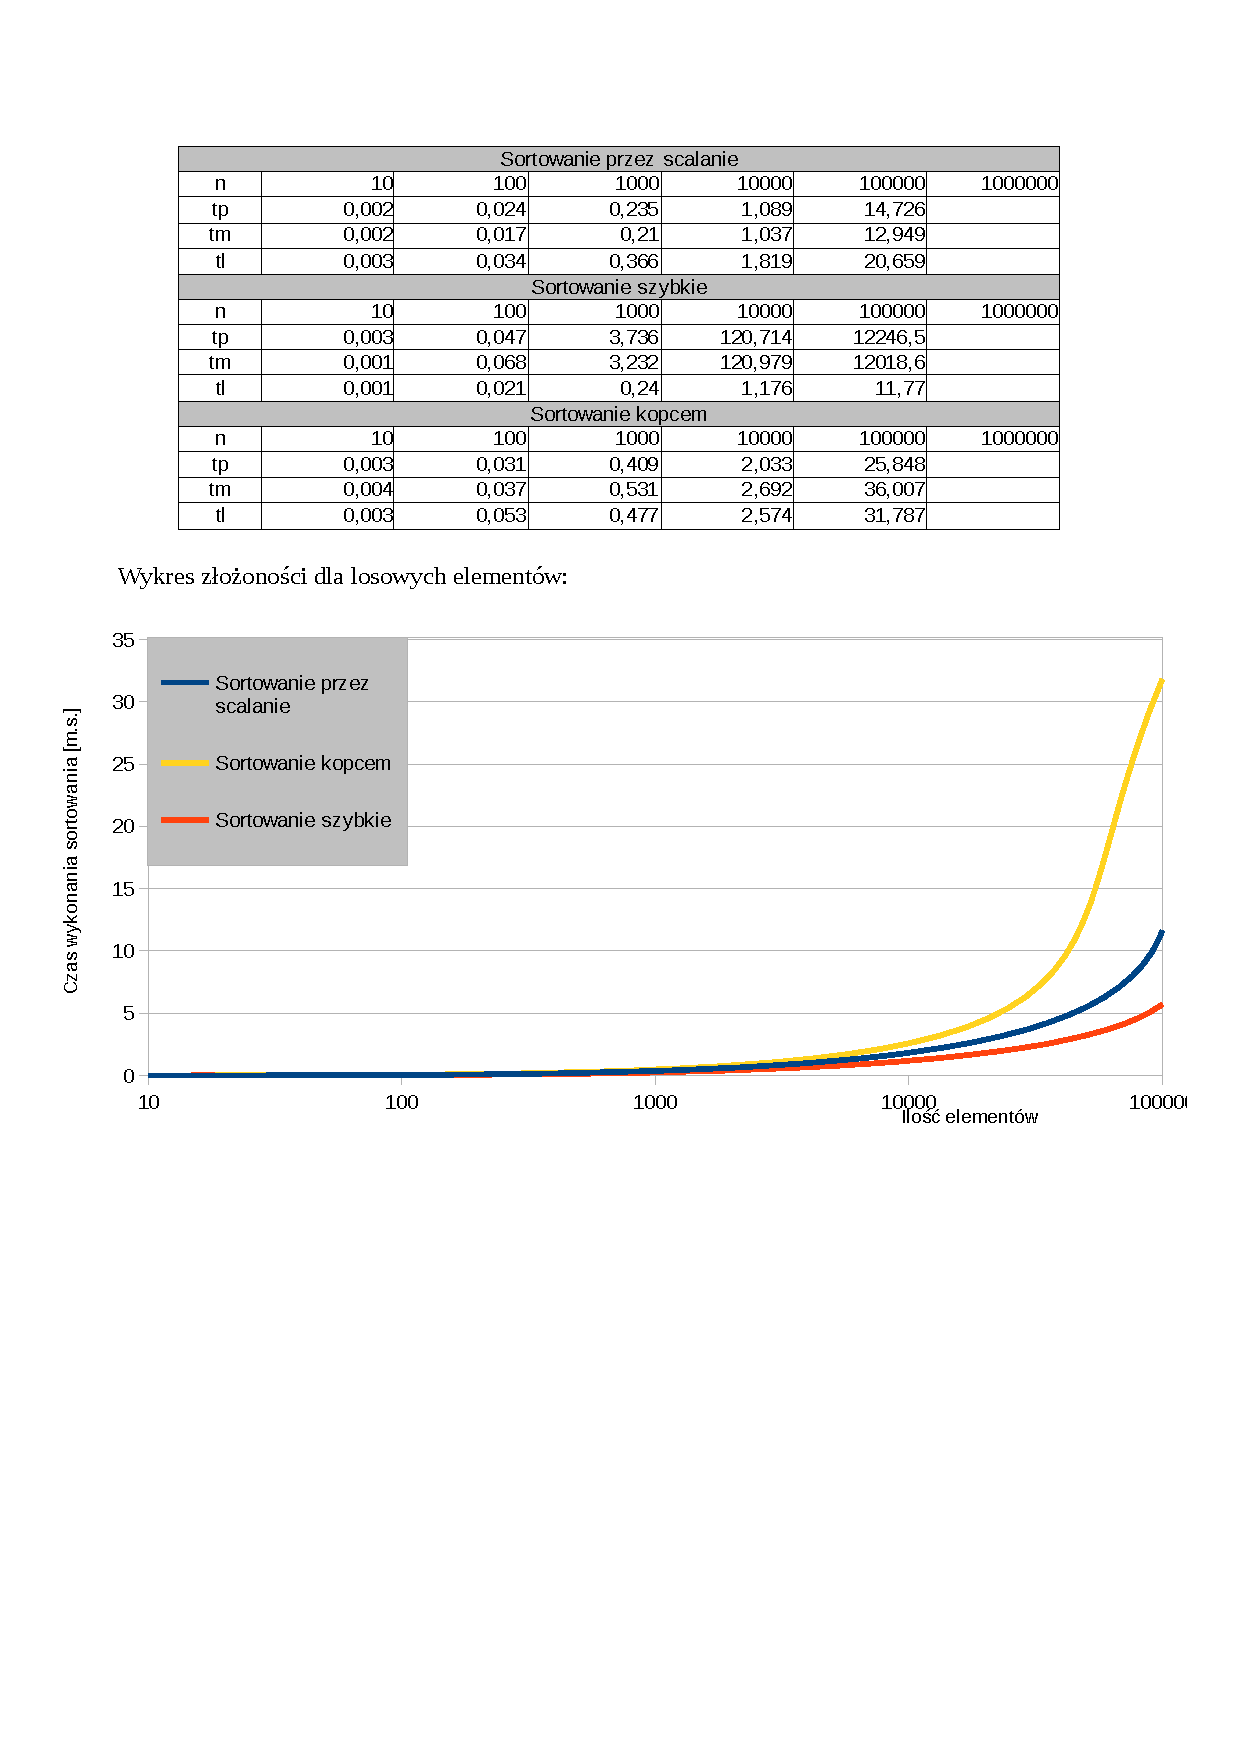
\includegraphics[width=\textwidth]{sort_czas1.pdf}
\label{fig:sort_czas1.pdf}
\end{figure}

\begin{figure}[H]
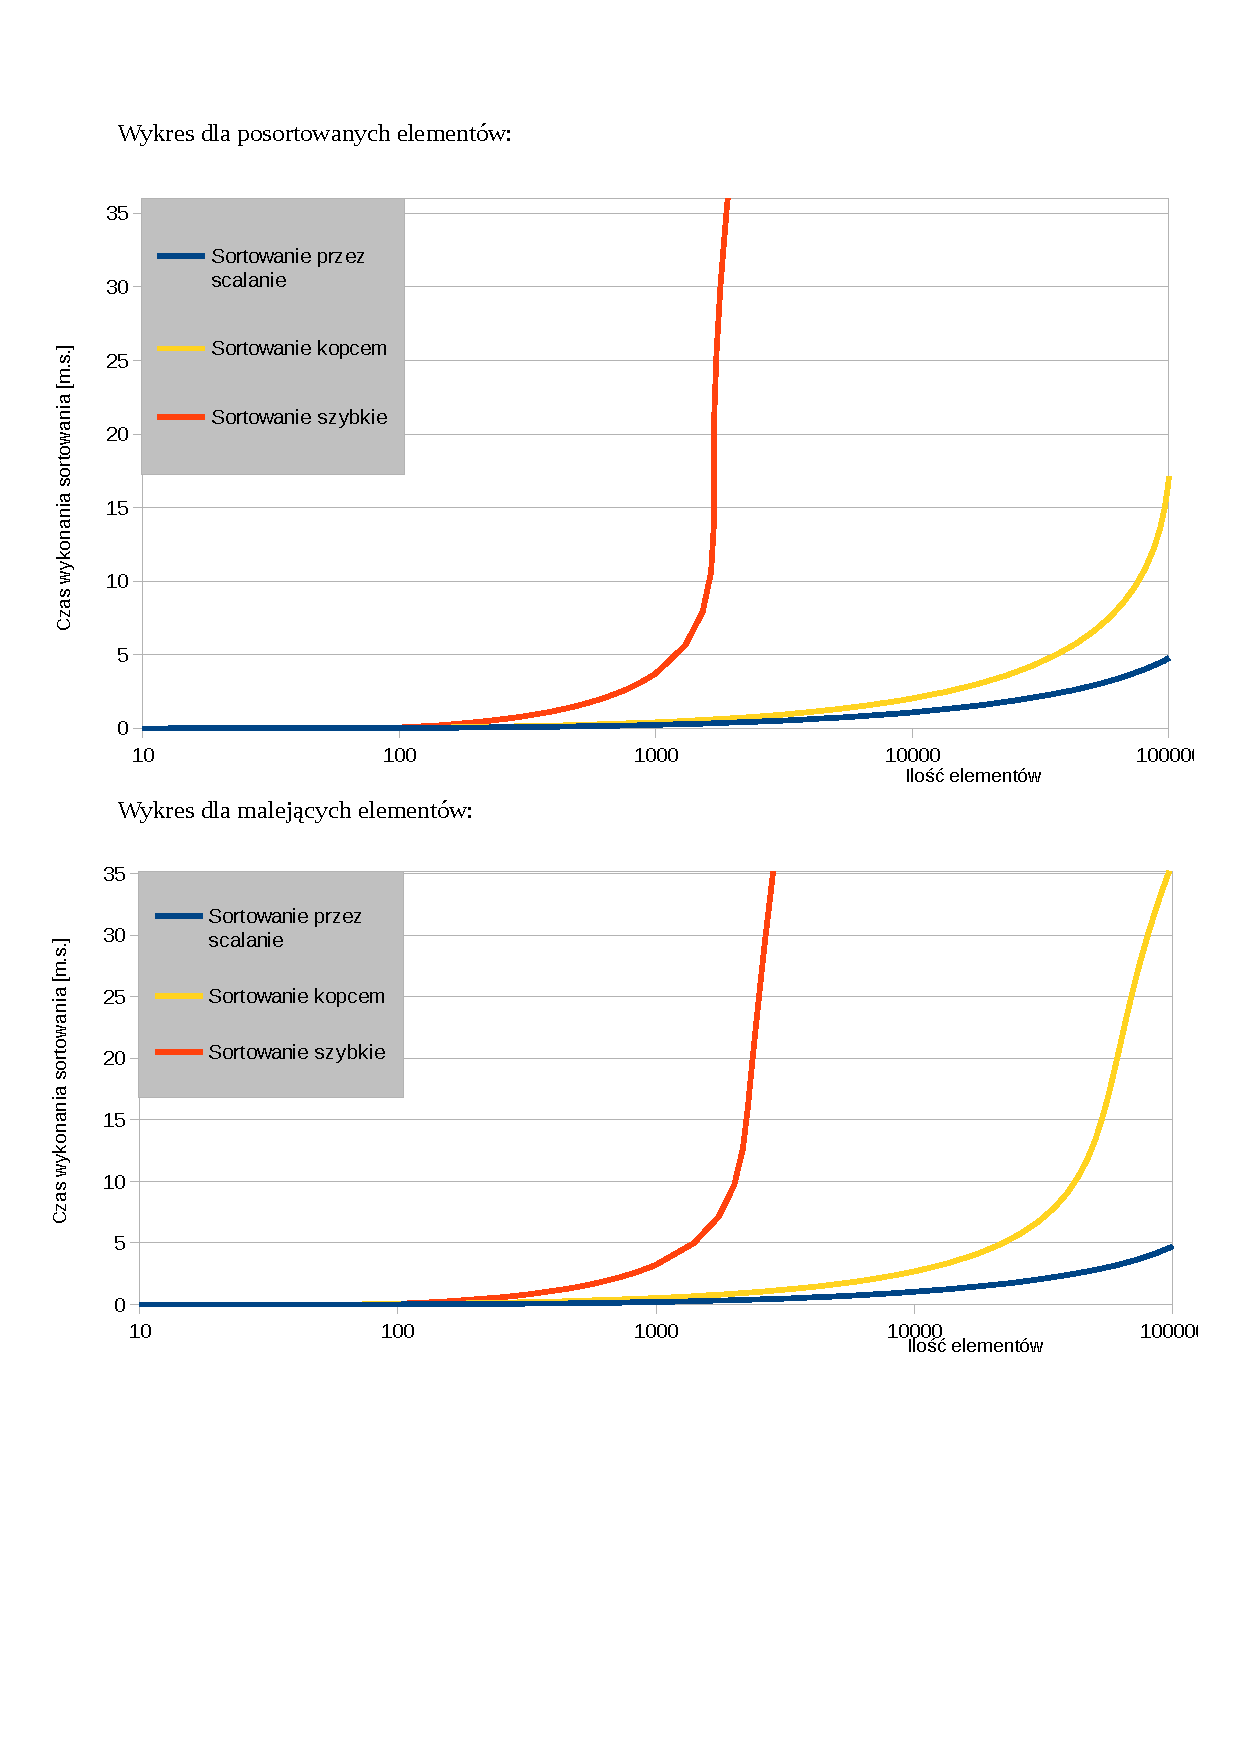
\includegraphics[width=\textwidth]{sort_czas2.pdf}
\label{fig:sort_czas2.pdf}
\end{figure}

\end{document}
